\subsection{Comparing the permutations}
The performance of the six different functions resulting from the possibilities of permuting mnk are tested with square matrices with memory footprints ranging from a few kB to hundreds of MB. The results are seen in figure \ref{fig:permGraph_none} with no compiler options. All six permutations perform equally well when the memory footprint is less than the L2 cache. For memory footprints larger than L2, the permutations with the loop over $n$ maintain the same performance, while the other four permutations have a significant reduction of performance. This is due to the fact that $m$ is the row index for matrices B and C, and that works well with the C language which is row major, meaning that the caches lines go along the rows of the matrices. The performance does not degrade after exceeding L3 which shows that program does not utilize the caches optimally. If that was the case, the smaller bandwidth between the memory and the processor would cause a significant drop in the performance when the memory footprint exceeds L3.
\begin{figure}
\centering
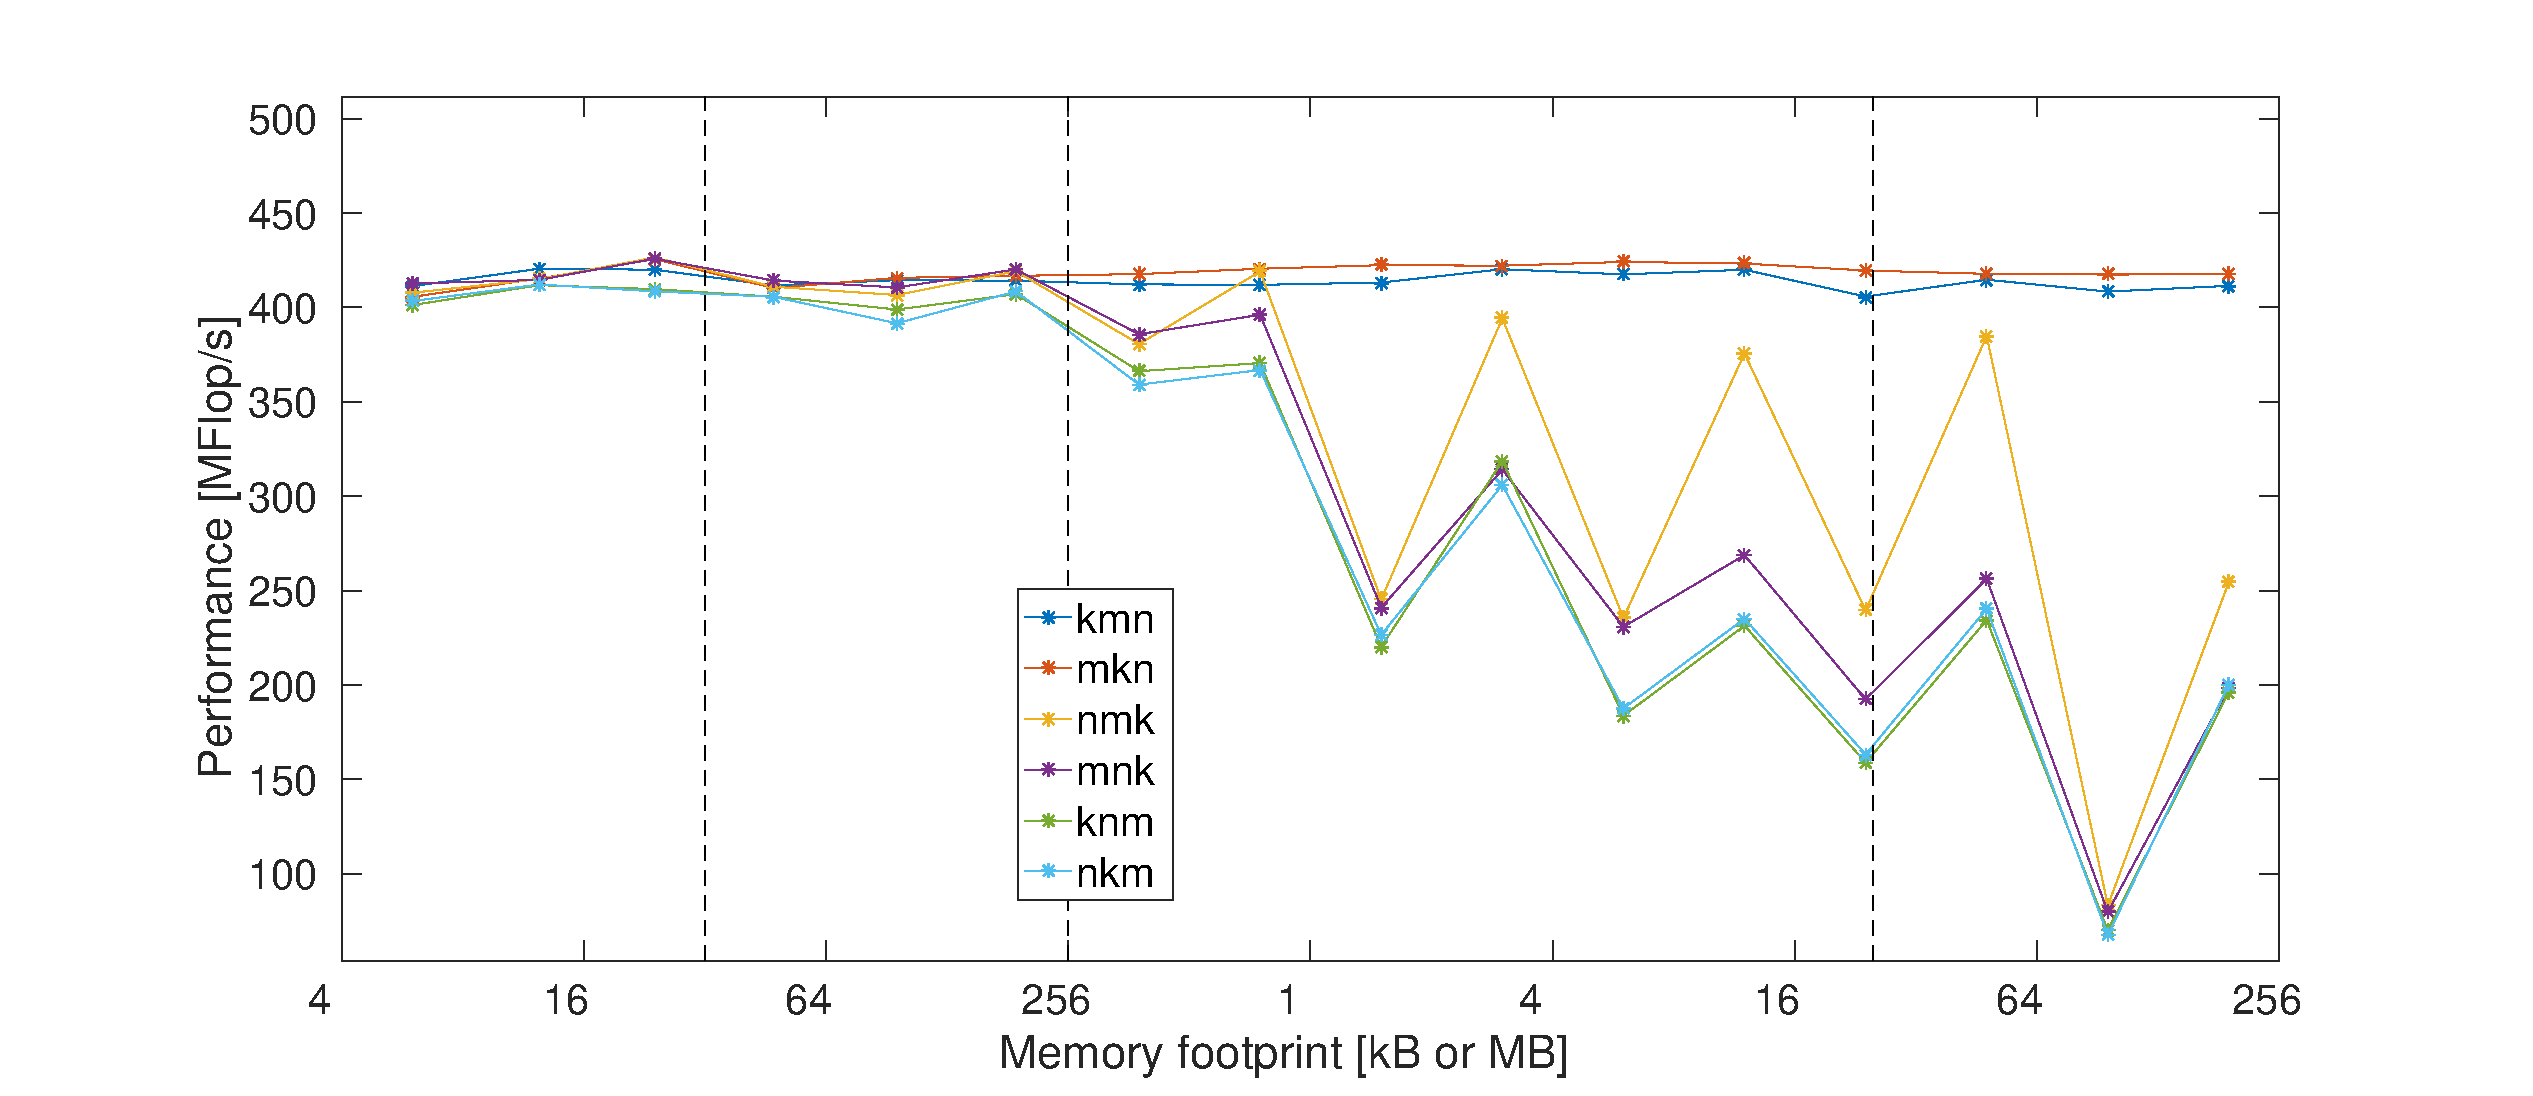
\includegraphics[width = 1.1\textwidth]{fig/permGraph_none.eps}
\caption{The performance of the different permutations versus the memory footprint, with L1, L2, and L3 caches shown as the vertical black dotted lines.}
\label{fig:permGraph_none}
\end{figure}
To investigate this, the same graph is produced, but this time the $\mathrm{-fast}$ option is activated in the Sun Studio compiler, and the results are shown in figure \ref{fig:permGraph_fast}. All six functions have improved performance compared to the case without compiler options, but the functions with $k$ as the inner loop, are a factor of $\sim 2$  slower for memory footprints which fit in either L1 and L2 caches. This is due to the fact that when $k$ is the inner loop, the program needs to fetch two new values to multiply together, and the compiler optimizer apparently has some issues optimizing this. When the memory footprint exceeds L2, the functions with $m$ as the inner loop drop off to the level of the functions with $k$ as the inner loop. This is because $m$ is the column size of matrices A and C, and looping over this as the inner loop goes against the row major format of C. For smaller memory footprints, the compiler is able to mitigate this issue, but after L2, the compiler optimizer can not fix the issue, and the performance drops. When the memory footprint does not exceed the size of the L3 cache, the performance of the functions with $n$ perform at a constant rate. This is again due to the row major format of C and $n$ being the row size of matrices B and C. After the L3 cahce size, the performance drops $\sim 10 \%$, which is less than expected, but that is probably due some extensive prefetching performed by the compiler when the $\mathrm{-fast}$ option is enabled. It is also worth noting that mkn performs better than kmn for all memory footprints, and the reason here is that the loop over $m$ is the slowest, and thus to achieve the best performance, this loop must placed as the outmost loop.

\begin{figure}
\centering
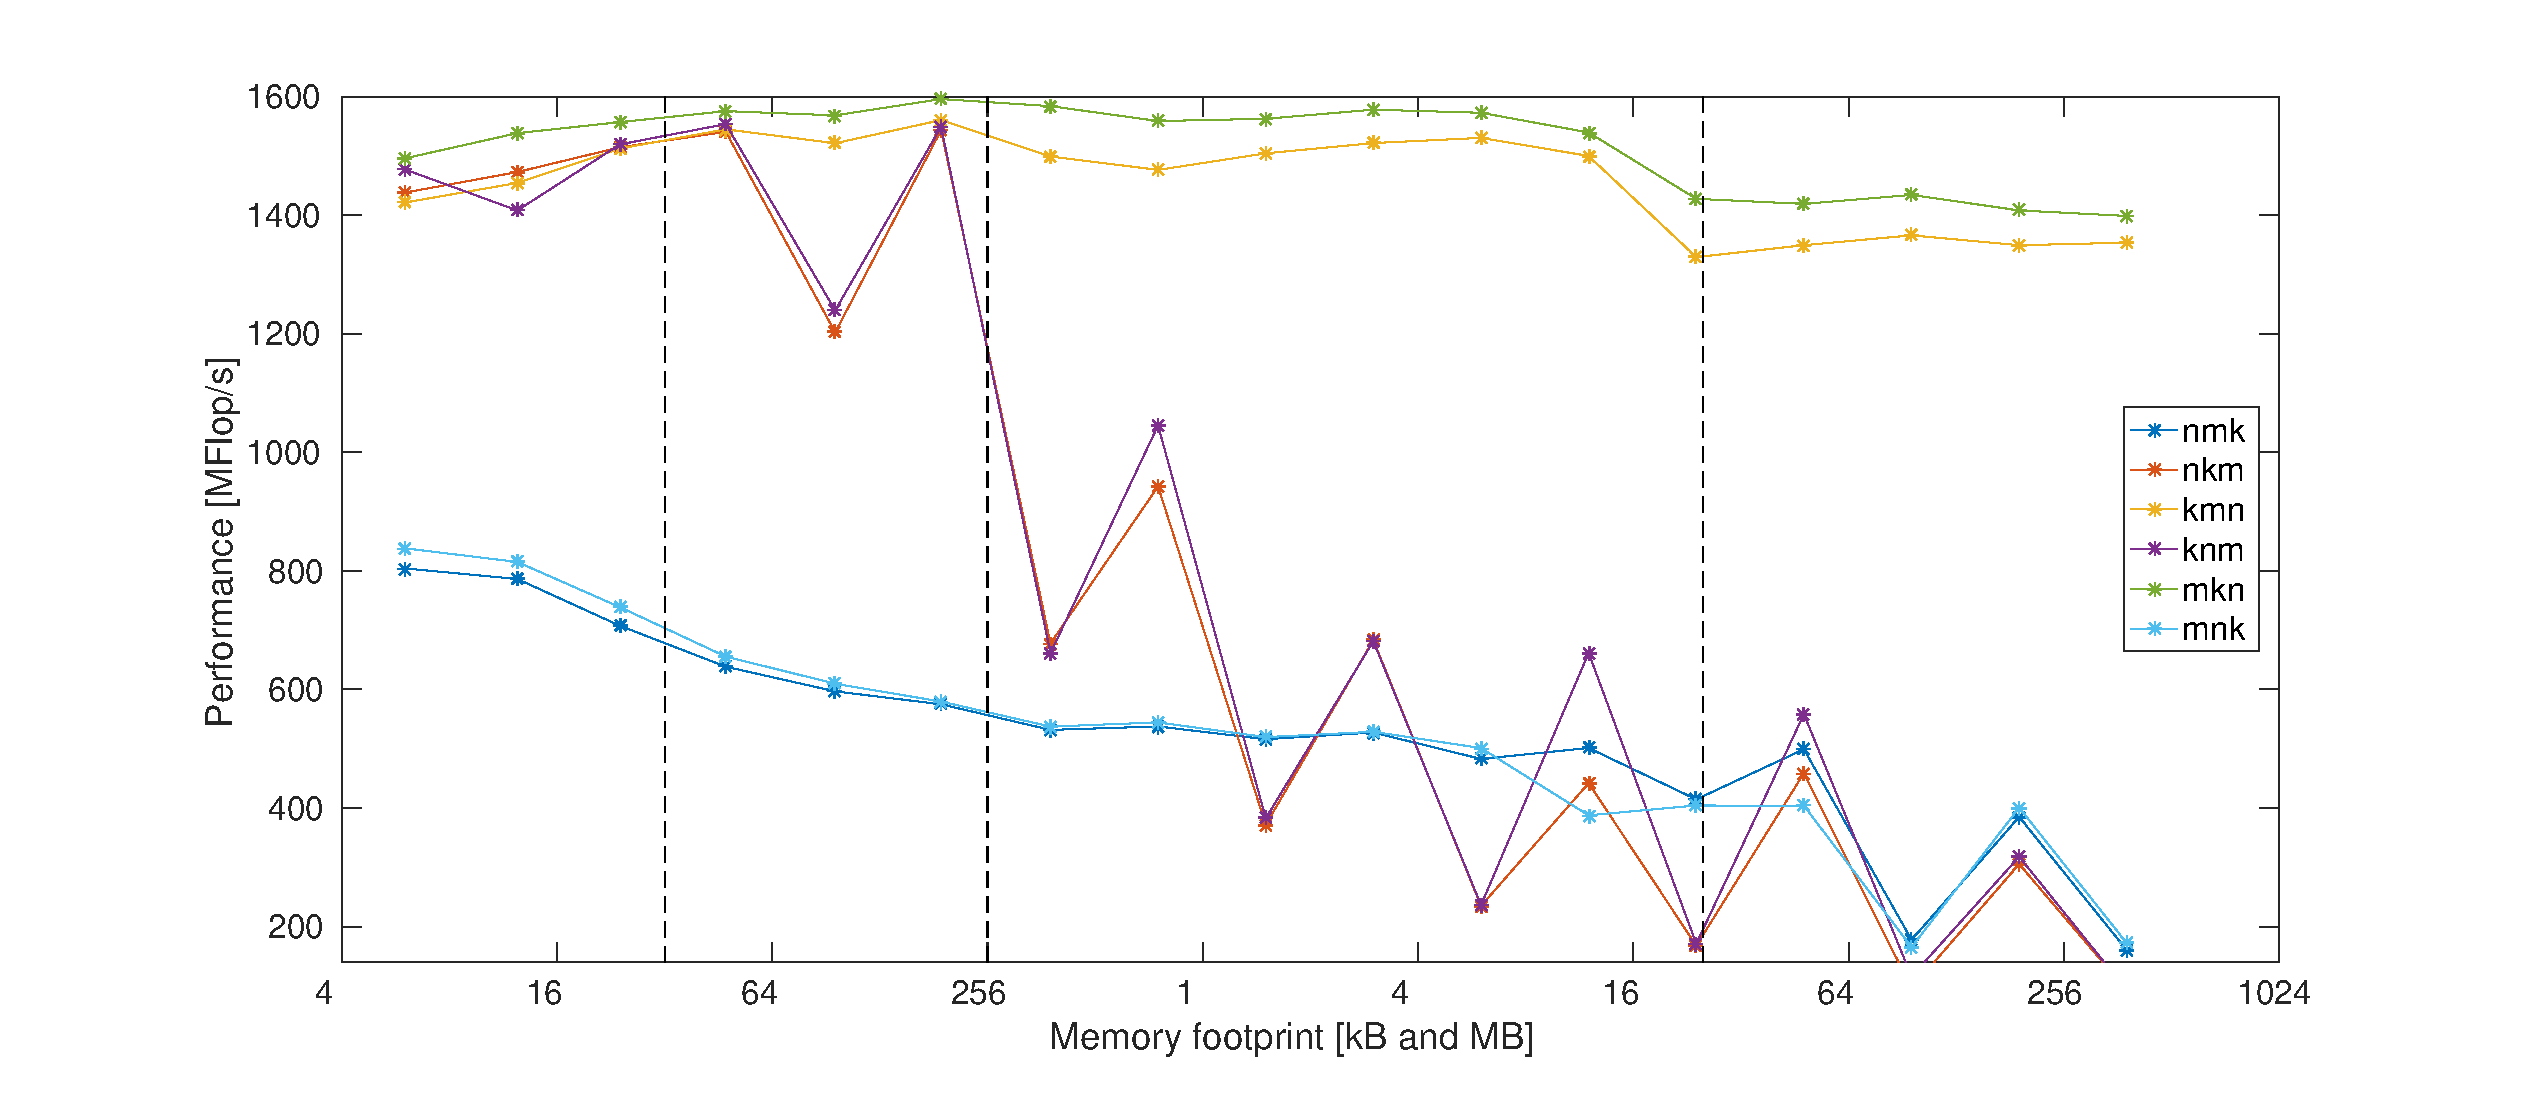
\includegraphics[width = 1.1\textwidth]{fig/permGraph_fast.eps}
\caption{The performance of the different permutations versus the memory footprint with compiler option $\mathrm{-fast}$ activated. L1, L2, and L3 caches shown as the vertical black dotted lines.}
\label{fig:comp1}
\end{figure}



\subsubsection{Analyzer tool}
We expect better-performing permutations to have less cache misses.   To validate our hypotheses regarding cache hits we conducted a profiling experiment. That is, we fixed the matrix dimension size to 724 which corresponds to ~12MB memory footprint, ran each of the six permutations (without compiler optimizations) using the collect command and viewed the results using Oracle Solaris Studio Performance Analyzer. To be able to make direct comparisons, we set the minimum runtime to zero and max iterations to one. This way each permutation is run for a single iteration and we can compare cache hits in absolute terms. \\
Level 1 and 2 cache hits and misses as well as CPU time of the permutations are presented in table \ref{tab:tab1}.
\begin{center}
\captionof{table}{Cache counters in millions with 12MB memory footprint} \label{tab:tab1} 
\begin{tabular}{ |c|c|c|c|c|c| } 
\hline
 & L1d hit & L1d miss & L2 hit & L2 miss & CPU time \\ 
\hline
nkm & 6849 & 755 & 704 & 50 & 2.410 \\  
\hline
nmk & 7229 & 373 & 373 & 1 & 2.030 \\ 
\hline
mkn & 7599 & 0 & 0 & 0 & 1.810 \\ 
\hline
mnk & 7229 & 376 & 328 & 47 & 2.310 \\ 
\hline
knm & 6849 & 755 & 704 & 51 & 2.350 \\ 
\hline
kmn & 7599 & 0 & 0 & 0 & 1.820 \\ 
\hline
\end{tabular}
\end{center}

Interpret results of table


When the memory footprint 



\begin{itemize}
\item hpcintro queue node cpu information
\item Introduce functions
\item Show library vs. native
\item introduce the permutations WITHOUT -fast and show the performance vs. memory footprint for all permutations
\item Optimize by compiler options (-fast, -O3, -prefetch etc. etc.)
\item Performace Analyzer tool experiment(s), relate results to  memory footprint-performance plot.
\item Blocking and find optimum block size
\item Compare blocking to the best w/o blocking
\end{itemize}
